
% Document Session
\documentclass{beamer}
\usetheme{Montpellier}
\title{Introdução à Séries Temporais: Modelos Lineares e Univariados}
\author{Marcos Ferreira}
\usepackage{enumerate}
\usepackage{graphicx}
\usepackage{multicol}
\graphicspath{ {./images/} }
\begin{document}
	%PACKAGES

	%FRAMES
	\frame{\titlepage}
	\frame{\tableofcontents}
	
	\section{Introdução}
	\subsection{Exemplos de Séries Temporais}
	\frame{
		\frametitle{Alguns Exemplos de Séries Temporais}
		\begin{enumerate}
			\item Valores diários de índice de poluição em São Paulo
			\item Valores \textbf{mensais} de média de temperatura na cidade de Cananeia 
			\item Índice \textbf{diário} da Bovespa ([B]\textsuperscript{3})
			\item Precipitação pluviométrica Acumulada,\textbf{Anual} em Fortaleza(acumulado anual)
			\item Número médio \textbf{anual} de Manchas Solares(acumulado de manchas no ano)
			\item Registro \textbf{contínuo} de tábua de Marés com um marégrafo 
			
		\end{enumerate}
	}
% poluicao
	\frame{
		\frametitle{Alguns Exemplos de Séries Temporais}
		% TODO: \usepackage{graphicx} required
		\begin{enumerate}
			\item \begin{figure}
				\centering
				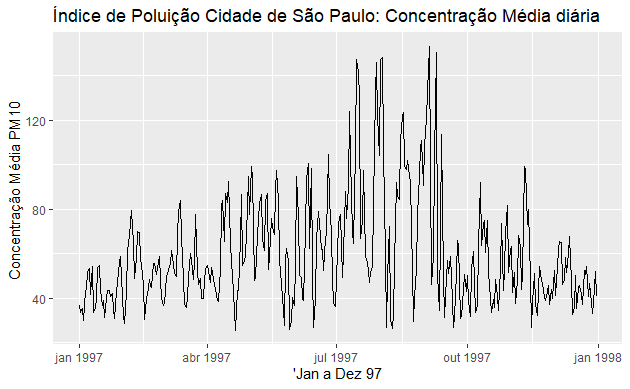
\includegraphics[width=0.7\linewidth]{apresentacao_series_temporais/images/Morettin_poluicao}
				\caption[Concentração de Poluentes - São Paulo : de 01/01/1997 à 31/12/1997]{Concentração de Poluentes - São Paulo : de 01/01/1997 à 31/12/1997}
				\label{fig:morettinpoluicao}
			\end{figure}
			
		\end{enumerate}
		
   }
\frame{
	\frametitle{Alguns Exemplos de Séries Temporais}
	% TODO: \usepackage{graphicx} required
	\begin{enumerate}
		\item \begin{figure}
			\centering
			\caption[Temperatura Média Cananeia : 1977 A 1985]{Temperatura Média Cananeia : 1977 A 1985}
			\label{fig:tempcananeia}
			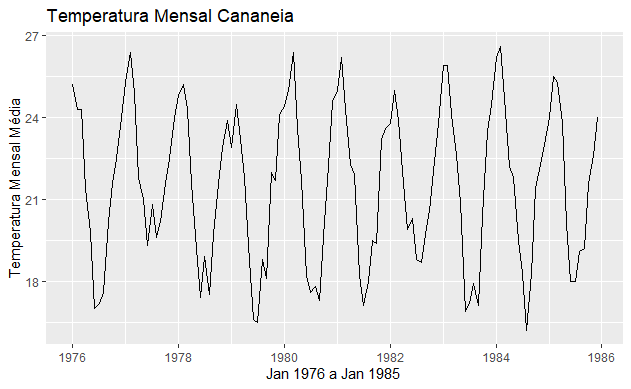
\includegraphics[width=0.7\linewidth]{apresentacao_series_temporais/images/temp_cananeia}
		\end{figure}
		
		
	\end{enumerate}
	
}
% bovespa 
\frame{
	\frametitle{Alguns Exemplos de Séries Temporais}
	% TODO: \usepackage{graphicx} required
	\begin{enumerate}
		\item \begin{figure}
			\centering
			\caption[Índice Diário Bovespa de 1998 à 2001]{Índice Diário Bovespa de 1998 à 2001}
			\label{fig:ibovespa}
			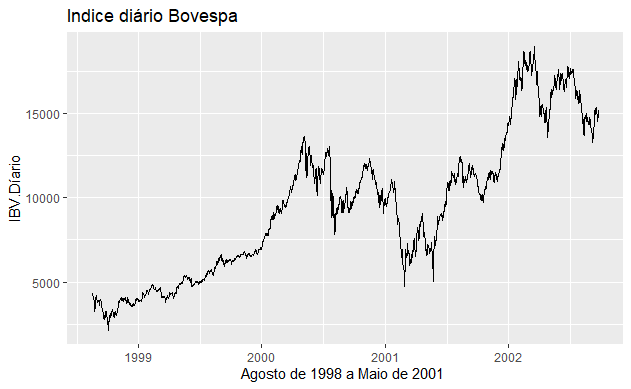
\includegraphics[width=0.7\linewidth]{apresentacao_series_temporais/images/IBOVESPA.D}
		\end{figure}
		
	\end{enumerate}
	
}



%Fortaleza - precipitaçaõa mm
\frame{
	\frametitle{Alguns Exemplos de Séries Temporais}
	% TODO: \usepackage{graphicx} required
	\begin{enumerate}
		\item\begin{figure}
			\centering
			\caption{Precipitação Pluviométrica média Anual Acumulada(mm) : Fortaleza (1849 a 1997)}
			\label{fig:fortaleza}
			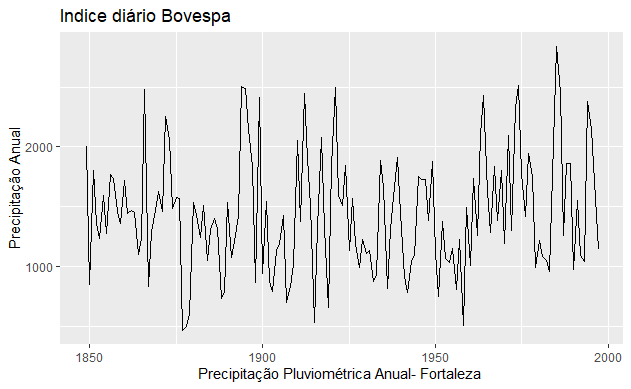
\includegraphics[width=0.7\linewidth]{apresentacao_series_temporais/images/Fortaleza}
		\end{figure}
		
		
	\end{enumerate}
	
}
% manchas
\frame{
	\frametitle{Alguns Exemplos de Séries Temporais}
	% TODO: \usepackage{graphicx} required
	\begin{enumerate}
		\item \begin{figure}
			\centering
			\caption{Número médio de Manchas Solares, desde 1749}
			\label{fig:manchas}
			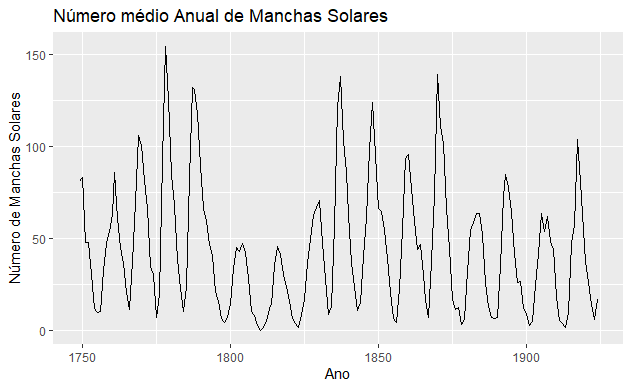
\includegraphics[width=0.7\linewidth]{apresentacao_series_temporais/images/manchas}
		\end{figure}
		
	\end{enumerate}
	
}

% PIB 
\frame{
	\frametitle{Alguns Exemplos de Séries Temporais}
	% TODO: \usepackage{graphicx} required
	\begin{enumerate}
		\item \begin{figure}
			\centering
			\caption{PIB ANUAL Preços de 1949}
			\label{fig:pib}
			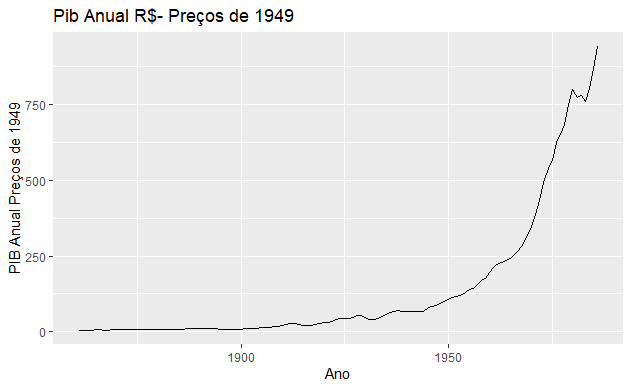
\includegraphics[width=0.7\linewidth]{apresentacao_series_temporais/images/pib}
		\end{figure}
		
		
	\end{enumerate}
	
}

\subsection{Considerações sobre as séries}
	\frame{
		\frametitle{Considerações}
		\begin{itemize}
			%
			\item<1-> Séries dos exemplos 1 a 5
			\begin{itemize}
				\item<1-> Séries temporais com domínio discreto	
			\end{itemize}
		    %
		    \item<1-> Série do exemplo 6
		    \begin{itemize}
		    	\item<1-> Série temporal com domínio de tempo continuo	
	   		\end{itemize}
   		   \item<1-> Uma série temporal com domínio de tempo discreto pode ser obtida através de uma amostragem, tomando-se os valores medidos a cada intervalo de tempo $\Delta t $
   		   \begin{itemize}
   		  	 	\item<1-> Por exemplo, no exemplo 6, podemos amostrar a altura da maré a cada uma hora, obtendo 24 pontos. O processo pode ser repetido no dia seguinte
   		   		\item<1-> Essa série terá 24 pontos em uma amostra de 1 dia 
   		   \end{itemize}
   		   %   			
		\end{itemize}
	}
\subsection{Enfoques para tratamento de série temporais}
	\frame{
		\frametitle{Dois Enfoques para Abordagem de Séries Temporais}
		\begin{itemize}
			\item<1-> Domínio Temporal
			\begin{itemize}
				\item<1-> Modelos Paramétricos
				\item<1-> Exemplo: Modelos ARIMA, na qual se estima os parâmetros dos valores do polinômio autoregressivo e de médias móveis, avaliando-se a significância de cada um deles				
			\end{itemize}
		\end{itemize}
		
		\begin{itemize}
		   	\item<1-> Domínio de Frequência( modelo não paramétrico)
		   	\begin{itemize}
			   	\item<1-> Consiste em decompor a série em componentes de frequência
		   		\item<1-> Exemplos:
		   		\begin{itemize}
		   			\item<1-> Análise Espectral
		   			\item<1->Aplicações em Física, Engenharia
		   		\end{itemize}	
		   	\end{itemize}
		\end{itemize}   	
		
			
	}
	% 
	\subsection{Objetivos da modelagem de séries temporais}
	\frame{
		\frametitle{Objetivos das Séries Temporais}
		\begin{itemize}
			\item<1-> Investigar o mecanismo Gerador da Série temporal
			\item<1-> Prever valores futuros da série, com base nos valores passados
			\item<1-> descrever o comportamento da série, usando-se, por exemplo, uma análise gráfica para averiguar tendências, ciclos, efeitos sazonais; analisar as correlações seriais, usando-se função de autocorrelação ou autocorrelação parcial(a ser visto adiante)
			\item<1-> Usar análise espectral de frequências para averiguar a periodicidade da série
		\end{itemize}
	}
	% 
	
\subsection{Transformação de Box-Cox}	
\frame{
	\frametitle{Transformações}
	\begin{itemize}
		\item<1-> Estabilizar a variância da série 
		\item<1-> Tornar o efeito sazonal aditivo 
		\begin{itemize}
		\item<1-> Tendências são comuns em séries financeiras e a variância pode aumentar, à medida que o tempo passa
		\end{itemize}
		 
		\item<1-> A transformação matemática das variáveis, principalmente a transformação logarítmica ajuda a 'estabilizar' a variância.
	\end{itemize}
}
\frame{
	\frametitle{Transformações: Transformações de Box-Cox()}
	\begin{itemize}
		\item<1-> $	Z_{t}^{(\lambda)} = 
		\begin{cases}
			  \frac{Z_{t}^{\lambda}-c}{\lambda}, se \lambda \neq 0,   \\
			
			 \log{Z_{t}}, & \mbox{ se } \lambda = 0
		\end{cases}
		$		
	\end{itemize}
	%
	\begin{itemize} 
		\item<1-> $\lambda$ e c são parâmetros a serem estimados
	\end{itemize}
	%
    \begin{itemize} 
    	\item<1->Essa transformação apropriada se o desvio padrão da série for proporcional à média , ( $\sigma \alpha \mu $)
    \end{itemize}

}
% Ferramentas 
\subsection{Alguns aplicativos para modelar séries temporais}
\frame{
		\frametitle{Ferramentas usadas em Séries Temporais}
		\begin{itemize}
			\item<1->  MINITAB
			\item<1->  SAS
			\item<1->  SPSS
			\item<1->  SPLUS
			\item<1->  Eviews
			\item<1->  Gretl
			\item<1->  R: Libraries astsa, forecast, tpp, GeneCycle, moments,stats,fbProphet
			\item<1->  Python: fbProphet, Arima, AutoArima\cite{morettin2018analise}
				
		\end{itemize}

}


\section{Modelos de Séries Temporais}
\subsection{Processos Estocásticos}
% capítulo 2
\frame{
	\frametitle{Processo Estocástico}
	\begin{itemize}
		\item<1-> Seja $\mathcal{T}$ um conjunto arbitrário \cite{morettin2018analise}\cite{enders2008applied}
		\item<1-> Um processo estocástico é :
		\begin{itemize}
			\item<1-> Uma família de variáveis aleatórias
			 \item<1-> $Z=\{\ Z(t), t \in \mathcal{T}  \}$
			 \item<1-> As variáveis aleatórias estão definidas em um espaço de probabilidades $(\Omega,\mathcal{A},\mathcal{P})$
			 \begin{itemize}
			 	\item<1-> $\Omega:$ espaço amostral
			 	\item<1-> $\mathcal{A}:$ Uma álgebra definida em $\Omega$
			 	\item<1-> $\mathcal{P}:$ Uma probabilidade, de modo que $\mathcal{P}(\Omega)=1$ 
			 \end{itemize}
		 \item<1-> $ \mathcal{T}$ definido em $\mathbb{Z}={\pm 1, \pm 2, \pm 3, ....}$ ou no conjunto dos reais $\mathbb{R}$
		\end{itemize}
	\end{itemize}

}
\subsection{Processos Estocásticos}
% capítulo 2
\frame{
	\frametitle{Exemplo de Um Processo Estocástico}
	\begin{itemize}
		\item<1-> \begin{figure}
			\centering
			\caption{Representação de um membro de uma família de um processo aleatório No eixo $f_{Z}$ temos a probabilidade de $Z(t)$ ; no eixo t, os elementos de $t \in \mathcal{T}$; e, finalmente na ordenadas, o valor de $Z(t)$ de um membro particular da família de processos estocástico; a curva $\mu(t)$ descreve a trajetória das médias de $Z(t)$ para cada t; finalmente, cada t pode ter uma distribuição de probabilidade diferente, embora o normal seja que a função de densidade de probabilidades seja a mesma.}
			\label{fig:familiadevariaveisaleatorias}
			\includegraphics[width=0.7\linewidth]{apresentacao_series_temporais/images/família_de_variaveis_aleatorias}
		\end{figure}
		
	\end{itemize}
	
}
\subsection{Especificação do Processo Estocástico em termos formais}
\frame{
	\frametitle{Especificação formal de um processo estocástico}
	\begin{itemize}
		\item<1-> Sejam $ {Z}^{(1)} ,{Z}^{(2)} , \dots$ realizações específicas da família de processos estocásticos
		\item<1-> Sejam agora, $t_{1},t_{2},\dots,t_{n}$ elementos quaisquer de $\mathcal{T}$
		\item<1-> Seja ainda, $F(z_{1},z_{2},\dots,z_{n}) = \mathit{P}( Z(t_{1}) \leq z_{1},Z(t_{2}) \leq z_{2},\dots,Z(t_{n}) \leq z_{n}   ) $
		\item<1-> $\mathit{P}$ é a probabilidade que cada $t_{i}$ seja menor do que $z_{i}$
		\item<1-> Se conhecermos as distribuições de probabilidade das variáveis aleatórias $Z(t_{i})$ o processo estará especificado, desde que $\mathit{P}$ satisfaçam as seguintes condições:
		\begin{itemize}
			\item<1-> Condição de simetria: para qualquer permutação $j_{1}, j_{2},\dots,j_{n}$ dos índices, então $F(z_{j_{1}},z_{j_{2}},\dots,z_{j_{n}}, t_{j_{1}},t_{j_{2}},\dots, t_{j_{n}}=F(z_{1},\dots,z_{n},t_{1},\dots,t_{n})$
		\end{itemize}
	\end{itemize}
}

\subsection{Especificação do Processo Estocástico em termos formais}
\frame{
	\frametitle{Especificação formal de um processo estocástico}
	\begin{itemize}
		\item<1-> Condição de Compatibilidade: se $m<n$ então $F(z_{1},z_{2},z_{m}; t_{1},t_{2},\dots,t_{m} )=F(z_{1},z_{2},z_{m},\infty;t_{1},t_{2},\dots,t_{m},t_{m+1},\dots)     $
	 \item<1-> Na prática, é difícil conhecer a especificação completa e o que se faz é estudar os momentos geradores do processo, em particular, os de baixa ordem
	 \begin{itemize}
	 	 \item<1-> Valor médio $\mu_{t}$
		 \item<1-> Variância $ \sigma_{t} $
	 	\item<1-> Covariância :$COV(X_{t},X_{s})=\gamma(t,s)$
	 \end{itemize}

	\end{itemize}
}

\subsection{Especificação do Processo Estocástico em termos formais}
\frame{
	\begin{itemize}
		\item<1->\begin{figure}
			\centering
			\caption{Representação de vários elementos de uma família de um processo estocástico Z, com realizações $Z^{(1)},Z^{(2)}, Z^{(3)},Z^{(4)}$}
			\label{fig:familiasvariaveisaleatorias2}
			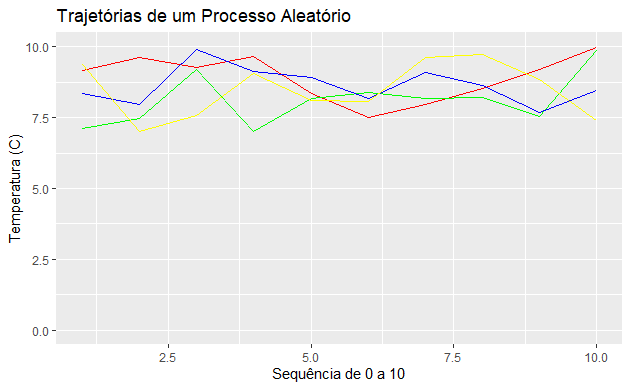
\includegraphics[width=0.7\linewidth]{apresentacao_series_temporais/images/familias_variaveis_aleatorias_2}
		\end{figure}
		
	\end{itemize}
}


\subsection{Processos Estacionários}
\frame{
	\frametitle{Processos Estacionários}
	\framesubtitle{Processos Estritamente Estacionários}
	\begin{itemize}
		\item<1-> Processos Estritamente Estacionários
		\begin{itemize}
			\item<1-> Um processo estocástico $Z =\{Z(t),t \in \mathcal{T}\}$ se suas estatísticas não são afetadas pela escolha da origem dos tempos ou devido à translação do tempo.
			\item<1-> Dito mais formalmente, todas as suas distribuições finito-dimensionais permanecem as mesmas sob translação no tempo, i.e:
			\begin{itemize}
				\item<1-> $\mathit{F}(z_{1},z_{2},\dots,z_{n}; t_{1}+ \tau, t_{2}+ \tau,\dots,t_{n}+ \tau,  )=\mathit{F}(z_{1},z_{2},\dots,z_{n}; t_{1}, t_{2},\dots,t_{n}  )$ 
			\end{itemize}
			\item<1-> As distribuições são invariantes sob uma translação. No caso de uma distribuição unidimensional com momentos finitos, então, a média e variância são constantes finitas, isto é:
			\item<1-> $\mu(t) = \mu ; V(t)=\sigma^{2}$
			\item<1-> As distribuições bidimensionais dependem de $t_{2} - t_{1}$ de modo que $\gamma(t_{1},t_{2})=\gamma(|t_{1}-t_{2}|)$
		\end{itemize}	
 	\end{itemize}
}
\subsection{Processos Estacionários}
\frame{
	\frametitle{Processos Estacionários}
	\framesubtitle{Processos Processos Fracamente Estacionários}
	\begin{itemize}
		\item<1-> Processos Fracamente Estacionários
		\begin{itemize}
			\item<1-> Um processo $Z=\{Z(t), t \in \mathcal{T}\}$ é dito fracamente estacionário ou estacionário de segunda ordem se e somente se:
			\item<1-> $E\{Z(t)\}= \mu(t)= \mu$; constante para todo $t\in \mathcal{T}$
			\item<1-> $E\{Z^{2}(t)\}\}< \infty $ para todo $t\in \mathcal{T}$
			\item<1-> $ \gamma(t_{1},t_{2}) =Cov(Z(t_{1},t_{2}))  $ é função de $|t_{1} - t_{2}|$
		\end{itemize}
		\item<1-> Em um processo fracamente estacionário, somente se requer condições sobre os momentos de primeira e segunda ordem e não sobre a função de distribuição finito-dimensional. \cite{fischer1982series} 
	\end{itemize}
}
\section{Função de Autocovariância}
\subsection{Autocovariância}
\frame{
	\frametitle{Função de Autocovariância}
	\begin{itemize}
		\item<1-> Define-se a função de autocovariâcia(facv) com defasagem $k$ da série como :
		\item<1-> $\gamma_{k}=Cov(Z_{t},Z_{t+k}) = E[(Z_{t}-\mu_{t})(Z_{t+k}- \mu_{t+k})]$
		\item<-1> Se a série é estacionária, então $\mu_{t}=\mu_{t+k}=\mu$
		\item<1-> Se a série for estacionária, então as seguintes propriedades são válidas para a função de autocovariância:
		\item<-1> $\gamma_{0}>0$
		\item<-1> $\gamma_{t}=\gamma_{-t}$
		\item<-1> $|\gamma_{t}|\leq \gamma_{0}$
		\item<-1> $\sum\limits_{j=1}^{n}\sum\limits_{k=1}^{n}{a_{j}.a_{k}.\gamma_{\tau_{j} -\tau_{k} }  } \geq 0, \forall a_{k}, a_{j}  \in \mathbb{R}$
		\item<-1> essa última propriedade define que $\gamma_{\tau}$ é não negativa definida
	\end{itemize}
	
}
\section{Referências}
\bibliography{./bibliografia}
\bibliographystyle{ieeetr}	
\end{document}